\section{Method}

% how the wsd proposed in this paper works:
% 	1. language model from wikipedia corpus
% 		-LDA & LSA
% 		-different dimensionalities
% 	2. labeled reference data
% 		-convert documents of reference data to topic vector space
% 		-save vector with sense id (=label)
% 	3. sense disambiguation
% 		-convert tested document to topic vector space
% 		-retrieve top k senseid using cosine measure from saved vector->senseid mapping
% 		-sense id of tested document is most frequent sense id in the top k retrieved
\thispagestyle{plain}

We created LSA, LDA and HDP topic models on the english wikipedia corpus (see \ref{creation}). To investigate the influence of topic count on the results, we  computed multiple instance of LDA and LSA models with different amounts of topics. Note that we do not include this step in our algorithm description - it is simply assumed that a trained topic model is already available.\\

Our algorithm consists of a training phase and an evaluation phase, however the training phase does not actually train a classifier. Instead, the contexts of all training instances are converted to the vector space of the topic model, and supsequently they are saved associated with the resepctive sense id.\\
The evaluation of a test instance is then done as follows. The test instance is also converted to the vector space of the topic model. Then, the top $k$ training contexts for the word in question are retrieved using the cosine similarity of the contexts. Finally, the sense id that occurs most frequently in the top $k$ results is chosen as the result for the test instance. Note that setting $k$ very high will simply result in always choosing the most frequent sense, which is in fact the baseline to which we measure the system's performance.\\

%initialize TM
%sense_vectors = Map()

%for each word in dictionary:
%	sense_vectors[word] = List()

%for each instance in train set:
%	vector = TM.convert(instance.vector)	
%	sense_vectors[instance.word].append(vector)
%

%for each instance in evaluation set:
%	candidates = sense_vectors[instance.word]
%	sort candidates by cosine similarity to TM.convert(instance)
% 	candidates = keep top k candidates
%	best_sense = most_frequent(candidates, k)
%	save this result
%
%
\begin{algorithm}[!t]
\caption{Word-Sense Disambiguation}\label{wsdalgorithm}
\begin{algorithmic}[1]
\State $\textit{initialize} \text{ TM} $
\State $\textit{sense\_vectors} := \textit{Map} {()}$
\Procedure{Train}{}
\ForAll {$instance \in train set$}
 \State$	vector := TM.convert(instance.bow)$
 \State$	l := sense\_vectors[instance.word]$
 \State$	l.append((vector, sense\_id))$
 
\EndFor
%\State \Return $D_{comp}\cup D_{inc}$
\EndProcedure
\Procedure{Evaluate}{}
\State $\textit{results} := \textit{Map} {()}$
\ForAll {$instance \in evaluation set$}
 \State$	vector := TM.convert(instance.bow)$
 \State$	candidates := sense\_vectors[instance.word]$
 \State	sort candidates by cosine similarity to vector
 \State	cut off candidates at index k
 \State$	best\_sense := most\_freq\_sense(candidates)$
 \State$	results[instance.id] := best\_sense$
 \State \Return $results$
\EndFor
%\State \Return $D_{comp}\cup D_{inc}$
\EndProcedure
\end{algorithmic}
\end{algorithm}

\subsection{Training of Topic Models}
\label{creation}
% details on data and how we created topic models
% 	1. wikipedia dumps
% 		-wikipedia does frequent dumps
% 		-we are using the latest dump of the articles in english wikipedia (as of june 2014) as xml
% 		-about 10GiB of compressed data, ~3.6 million documents
% 	2. topic model creationg
% 		-using gensim python library (decription of library)
% 		-gensim usage: lsa/lda interface, paramter description
% 		(-description of calculation time and machine hardware)
% 	3. additional models
% 		-hdp as test, implementation not mature therefore just used as test case
% 		-other models provided by gensim (random projections, log entropy) not used

For the training of a topic model large amounts of text are required. For providing that data we looked at the English Wikipedia. Wikipedia does frequent backups of its articles and provides them for public use. We used the latest dump (June 2014) containing about 10GiB of compressed XML data, or 3.6 million documents \cite{wikidumps}. The topic models were all trained using this data in an unsupervised manner.\\\\
The implementations of LSA, LDA and HDP topic models that we used were all provided in the python library gensim. Gensim is a free, open-source library for topic modelling. For using the wikipedia dump with gensim, it first had to be preprocessed using TF-IDF. Gensim was then used to create LSA, LDA and HDP models with different levels of dimensionalities from that corpus. We did not stem our training data, as this would have been very computationally expensive. In evaluation, the context data was therefore also not stemmed.\\\\
There are other models that are also supported by gensim that were not used for different reasons. Random projections (RP) \cite{RandomProjections, gensimRP} and log entropy (LE) \cite{LogEntropy, gensimLE} models were not used due to time contraints, but also because we did not expect them to outperform our other models. LE does not perform any dimensionality reduction, and RP does not usually outperform LSA. 


\thispagestyle{plain}


\section{Experiments}
\subsection{Experimental Setup}
We used the SensEval-3 English lexical sample data as our training and evaluation set, so that we would be able to compare the performance of our approach to existing systems. The baseline performance for this task is to always choose the most frequent sense for each word.\\\\
We ran a large number of experiments at different parameters in order to find the optimal model and configuration. LSA was evaluated at $n=$150, 200, 250, 300, 350 and 400 topics, each with a single pass over the corpus, two power iterations and no decay.\\\\
LDA was only evaluated at 200, 300 and 400 topics, since it is more computationally expensive to create those models. Here we used a symmetric prior of $\alpha = \frac{1}{n}$ for the per-document topic distribution, with the same value for $\beta$, the per-topic word distribution.\\\\
HDP was evaluated using the default parameters of Gensim: $\kappa = 1, \tau = 64, \alpha =1, \gamma =1, \eta =0.01$. Unfortunately, we were not able to properly use the HDP model, as the topics it generated did not appear make sense, and were all nearly identical. Due to time constraints we were not able to fix these issues and retrain the model. The results are nevertheless included in this paper.\\

\subsection{Results}
Figure~\ref{fig:lsa}, Figure~\ref{fig:lda} and Figure~\ref{fig:all} visualize the results we obtained for different dimensionalities of LSA and LDA. The failed HDP attempt is not included (it was in fact lower than the baseline performance). \\
\begin{figure}
   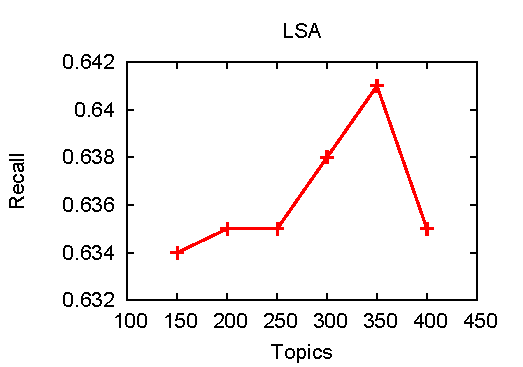
\includegraphics{plot/lsa_lines.pdf}
  \caption{LSA results}
  \label{fig:lsa}
\end{figure}

\begin{figure}
  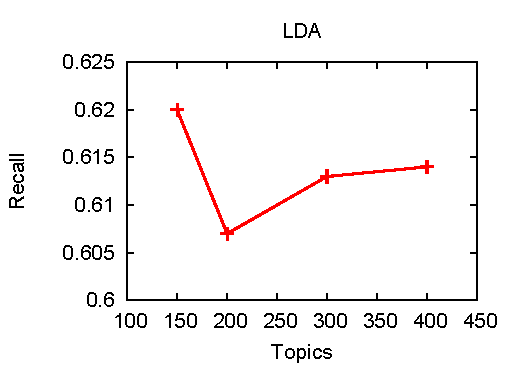
\includegraphics{plot/lda_lines.pdf}
  \caption{LDA results}
  \label{fig:lda}
\end{figure}

\begin{figure}
  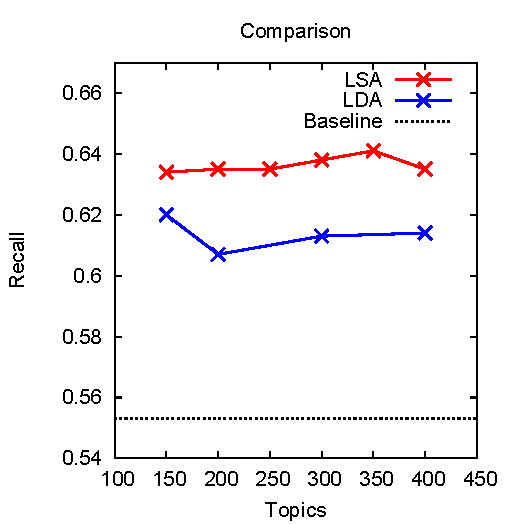
\includegraphics{plot/joined_baseline.pdf}
  \caption{Comparison of results and baseline}
  \label{fig:all}
\end{figure}
As you can see, LSA outperforms LDA, and achieves its highest result of 64.1\% at 350 topics with $k=10$. The best performance for LDA was a recall of 62\% at 150 topics. The HDP model only achieved a recall of 47.4\%, which is below baseline performance (which is possible as only values of k below 50 were considered). Other systems in SensEval-3 ranged from approximately 60\% to 73\% recall\cite{senseval3paper}, so while our system is not on par with the state of the art in its current form, it performs reasonably well and presents a decent approach to the presented task. 


\subsection{Outlook}
The algorithm presented here was fairly primitive, and serves mainly as a benchmark to compare the performance of different topic models for WSD. To optimize the systems performance, additional features may be considered and used to train a classifier of some sort. The entry \textit{IRST-Kernels} by the Team ITC-IRST at SensEval-3 was one of the highest performing systems, and used LSA in conjunction with paradigmatic and syntagmatic information and other features in an SVM classifier\cite{senseval3paper}. It is conceivable to achieve significantly higher performance by following similar methods, especially by considering local features in conjunction with LSA (which ignores local features).\\\\
There are also many more topic models that can be tried, as well as parameters in the training that can be tweaked. Going beyond topic models, any dimensionality reduction algorithm could be applied to this approach of WSD. For example, an interesting method to consider might be marginalized Stacked Denoising Autoencoders (mSDA), which actually come from the field of deep learning but have in some benchmarks outperformed LDA in both accuracy and computational complexity.
% how did we score the diffent models
% 	1. scoring script provided, runs on test set, gives f-score/recall
% 	2. plotting tools / how were the graphics generated
% 	3. plot data: dimensionality against f-score
% 	4. interpretation of plots: what does that mean, how well did it perform



